\newpage
\section{Architecture du réseau}

\subsection{Pré-traitement des données:}
    Nous effectuons plusieurs pré-traitements des données de séquence et mot cible.
    \subsubsection{Vectorisation}
        Le premier pré-traitement consiste à ne garder que la dynamique de mouvement plutôt que de coordonnées des séquences. C'est pourquoi nous avons choisis une représentation vectorielle plutôt que sous forme de coordonnées tel que :
        $v(i)=\left\{\begin{array}{l}x(i+1)-x(i) \\ y(i+1)-y(i)\end{array}\right.$
    
    \subsubsection{Remplissage}
        Afin de traiter les données en lots il est nécessaire qu'elles aient la même taille. C'est pourquoi nous utilisons des techniques de remplissages afin que les séquences d'entrées et sorties possèdent toutes la taille maximale qui existe dans l'ensemble de donné.
        \newline 
        Le remplissage de la séquence d'entrée se fait en remplissant de (0,0) les vecteurs. Cela signifie qu'il n'y a plus de déplacement du stylo et reviendrait à répéter plusieurs fois les coordonnées du dernier points. 
        \newline
        Le pré-traitement des mots cibles se fait en ajoutant un symbole d'arrêt ainsi qu'un symbole de remplissage jusqu'à obtenir un mot de 6 lettres(5 lettres + symbole d'arrêt), en sachant que nous avons au maximum des mot de 5 lettres.

\subsection{Architecture choisie:}
    Pour répondre à cette problématique nous avons commencé par utiliser l'architecture de base de la traduction vu en cours :
    \begin{figure}[!ht]
        \centering
        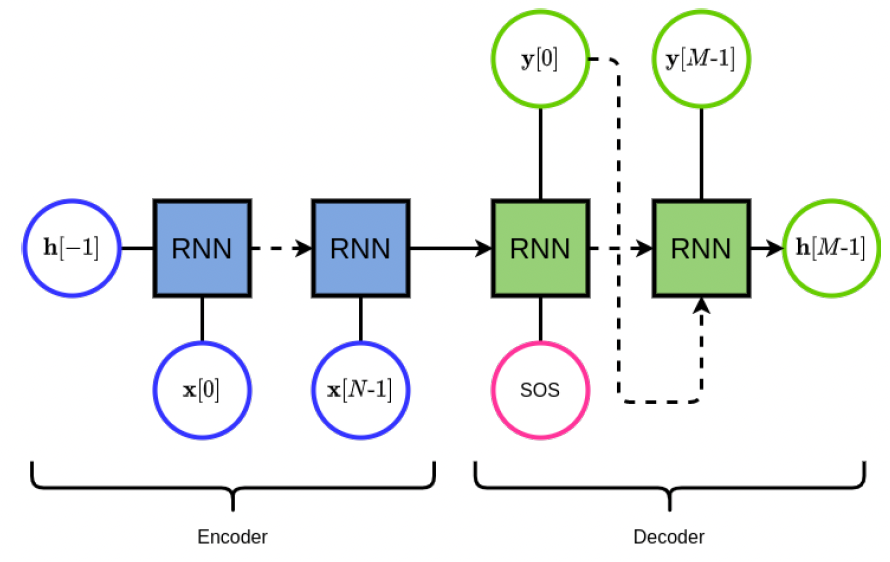
\includegraphics[width=80mm]{sections/images/architecture/traduction.png}
        \caption{Architecture de base de la traduction}
        \label{fig:Figure 2  }
    \end{figure}
    
    
    \subsubsection{unité d'Elman}
        Nous avons ensuite essayé les différentes unités de réseau de neurone récurrent tel que Elman, GRU et LSTM. Dans un premier temps nous remarquons un apprentissage difficile lors des premières itérations. Il semble que nous arrivons à un minimum local, cela est visible par l'apparition d'un plateau sur la courbe (\ref{fig:Figure 3  }) de loss et de distance entre 25 et 50 itérations. Néanmoins, l'apprentissage se poursuit correctement après la 75ème itérations.
    
        \begin{figure}[!ht]
        \centering
        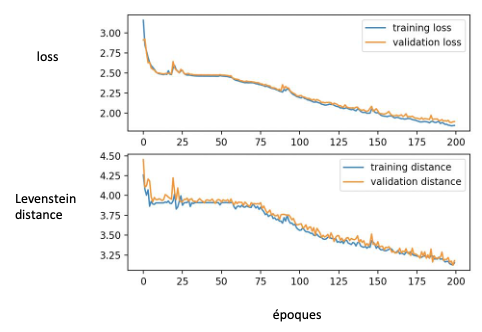
\includegraphics[width=80mm]{sections/images/architecture/RNN.png}
        \caption{Évolution de la fonction de coût et de la distance au cours des itérations pour Elman}
        \label{fig:Figure 3  }
        \end{figure}
        
    
    \subsubsection{unité LSTM}
        Nous avons pu observer de meilleures performances en utilisant GRU et LSTM qui effectuaient un apprentissage plus rapide qu'en utilisant des unités d'Elman. Le LSTM quant à lui semblait stagner et tomber plusieurs fois dans des minimums locaux. (Figure \ref{fig:Figure 4  })
    
        \begin{figure}[!ht]
            \centering
            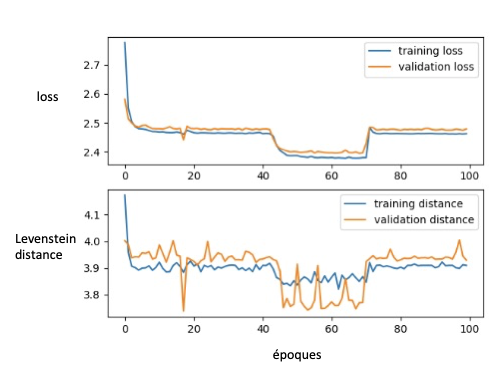
\includegraphics[width=80mm]{sections/images/architecture/LSTM.png}
            \caption{Évolution de la fonction de coût et de la distance au cours des itérations pour la LSTM}
            \label{fig:Figure 4  }
        \end{figure}
        
    \subsubsection{Unité GRU}
        Enfin entre le GRU quant à lui nous donnait les meilleurs résultats pour un faible nombre d'époque (100 époques). Cette différence peut être du au fait que le GRU utilise moins de paramètres que le LSTM et donc utilise moins de mémoire et s'exécute donc plus rapidement que le LSTM. La mémoire à long terme du LSTM lui permettrait d'être plus performant sur des séquences plus longues.
    
        \begin{figure}[!ht]
            \centering
            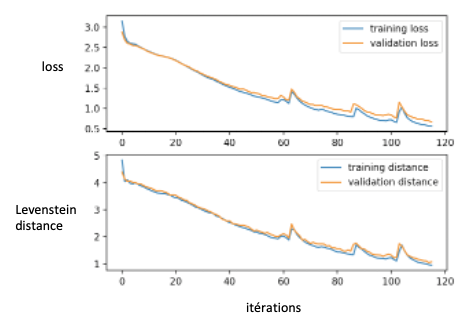
\includegraphics[width=80mm]{sections/images/architecture/GRU.png}
            \caption{Évolution de la fonction de coût et de la distance au cours des itérations pour la GRU}
            \label{fig:Figure 5  }
        \end{figure}

    \subsubsection{Module d'attention}
        
        Le module d'attention permet au réseau de se concentrer seulement sur certaines parties de la séquence d'entrée lors de la prédiction d'une lettre. Le but est d'utiliser de contexte a afin d'aider la classification de la lettre. 
        
        \begin{figure}[!ht]
            \centering
            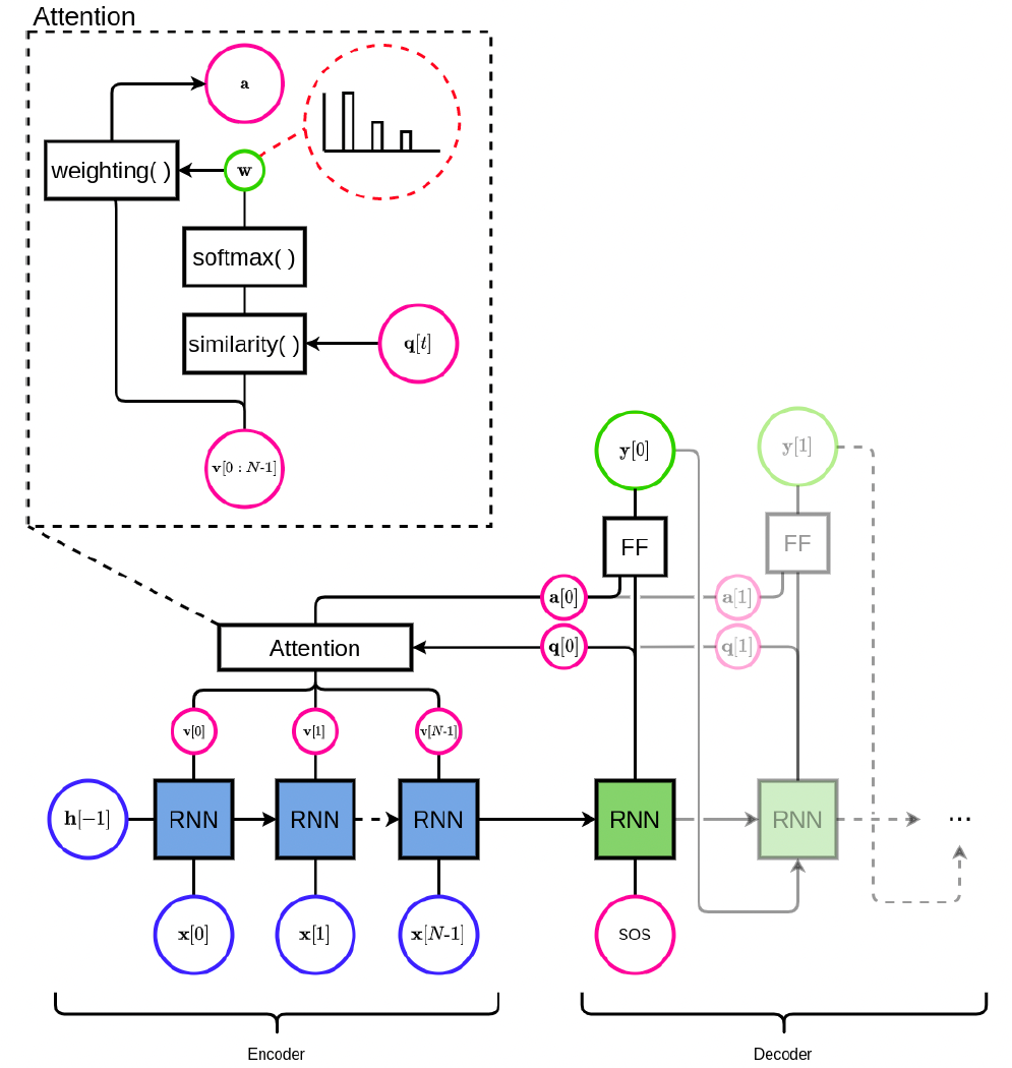
\includegraphics[width=80mm]{sections/images/architecture/attention_base.png}
            \caption{Module d'attention}
            \label{fig:Figure 6  }
        \end{figure}
        
        Pour se faire nous comparons dans un premier temps la sortie de l'encodeur à celle du décodeur en faisant passer préalablement la sortie du décodeur dans une couche entièrement connectée de dimension H\footnote{H : Taille de la couche cachée 23 \label{H}}. Cela nous donne au vecteur q[t] de dimension(B\footnote{B : Taille du batch à 100 \label{B}},1,H). La sortie du décodeur V est directement utilisée pour le calcul de la similarité et est de dimension (B,N\footnote{N : Taille maximum de la séquence \label{N}},H). La fonction de similarité choisie est celle du cosinus, nous avons fait se choix afin de réduire le nombre de paramètre à apprendre. Les valeurs en sortie du cosinus sont ensuite envoyées dans une fonction softmax() afin de déterminer les poids d'attentions w de la séquence tel que :
        
        \begin{align}
            \tilde{w_{i}}=\mathrm{cos}\left(\mathbf{v_{i}},q[t]\right), i \in N \\
            w_{i}=\frac{\exp \left(\tilde{w_{i}}\right)}{\Sigma_{k=0}^{N-1} \exp \left(\tilde{w_{k}}\right)} \\
            dim(\tilde{w})=dim(w)=(B,N,1)
        \end{align}
        
        La fonction weithing() permet de faire la somme pondérée des poids tel que :
        
        \begin{align}
            \tilde{a}=\mathbf{v}*w \\
            dim(\tilde{\tilde{a}})=(B,N,H) \\
            a=\Sigma_{k=0}^{N-1} \tilde{a_{k}}\\
            dim(a)=(B,1,H)
        \end{align}
        
        La somme (6) est faite sur la dimension 1. Nous obtenons donc en sortie un tenseur de dimension (B,1,H) (7) de même dimension que q[t]. Nous faisons ensuite la concaténation de q et a et nous obtenons un nouveau tenseur de dimension (B,2H) qui sera ensuite envoyé le FF (Feed forward (\ref{fig:Figure 7  })) composé de deux couches pleinement connectées. La première couche Att est de dimension (2H,H) et la deuxième couche est de dimension (H,D\footnote{D : Taille du dictionnaire de sortie (29 symboles) \label{D}})
        
        \begin{figure}[!ht]
            \centering
            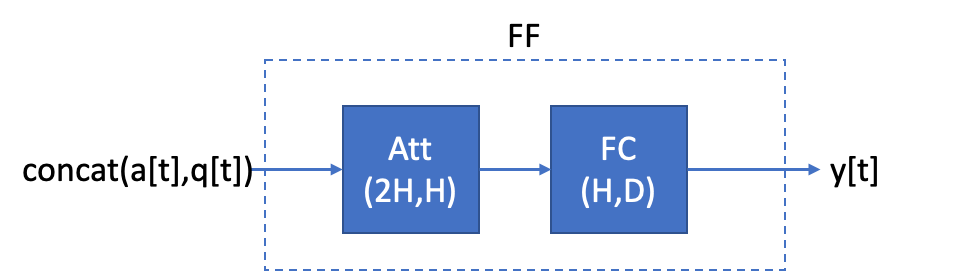
\includegraphics[width=80mm]{sections/images/architecture/sortie_att.png}
            \caption{Sortie du module d'attention}
            \label{fig:Figure 7  }
        \end{figure}
        
    \subsubsection{Réseaux récurrents bidirectionnels}
        Nous avons accès à la séquence d'entrée complète, il est donc possible d'utiliser des unités bidirectionnelles. Son usage s'avère efficace car elle nous permet d'accélérer grandement l'apprentissage et améliore nos résultats jusqu'à avoir du sur-apprentissage. Nous utiliserons des unités bidirectionnelles uniquement en entré du réseau car nous n'avons pas accès au éléments futur de la séquence de sortie puisque nous la générons un élément à la fois.
        
        \begin{figure}[!ht]
            \centering
            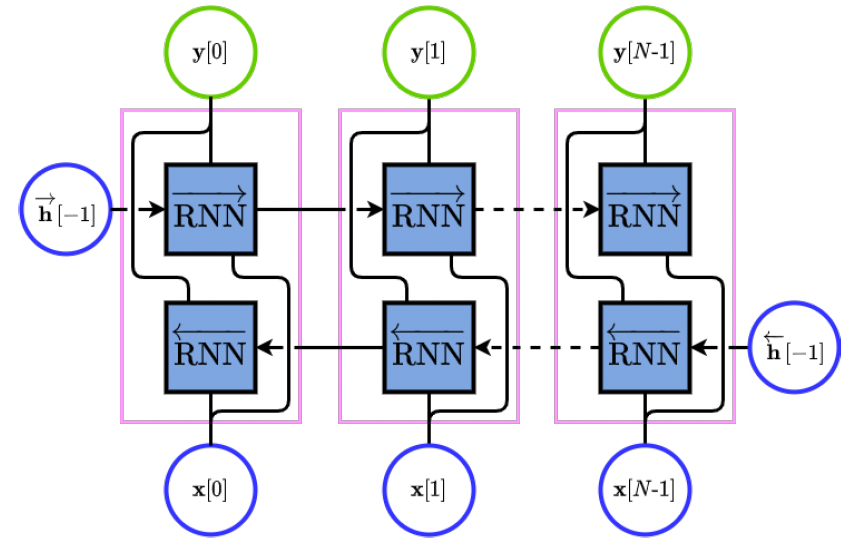
\includegraphics[width=70mm]{sections/images/architecture/bidirection.png}
            \caption{réseau de neurone bidirectionnel}
            \label{fig:Figure 8  }
        \end{figure}
        
        Lors de l'utilisation de la bidirectionnalité les dimensions du tenseur de sortie du décodeur V change et deviennent (B,N,2H). Nous adaptons le reste du réseau tel que :
        \begin{itemize}
            \item La couche précédent q passe de dimension (H,H) à (H,2H) afin d'avoir q[t] de dimension (B,2H).
            \item La couche Att passe de dimension (2H,H) à (3H,H).
            \item Doubler le nombre de couche n du décodeur (2*n couches).
        \end{itemize}
\newpage
\subsection{Schéma-bloc des couches du réseau :}
    
    Avec l'architecture suivante nous cumulons 32747 paramètres à entraîner.
    
    \begin{figure}[!ht]
            \centering
            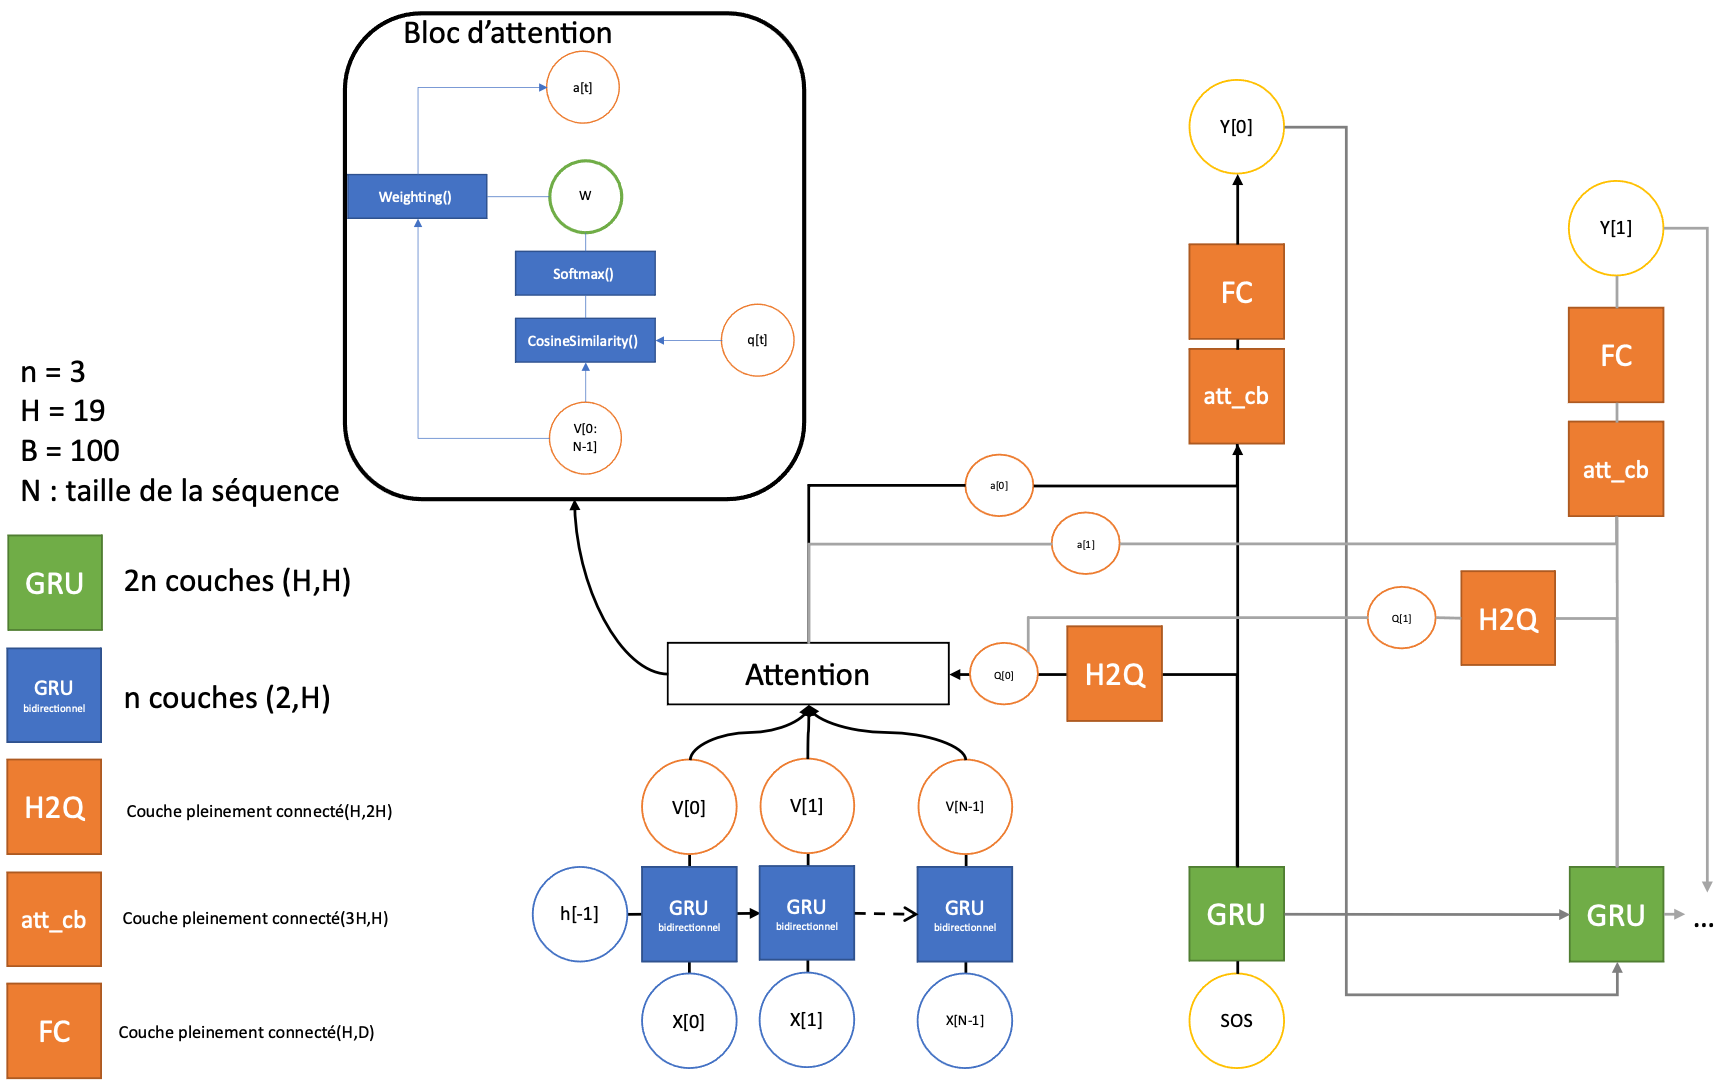
\includegraphics[width=150mm]{sections/images/architecture/schameBloc.png}
            \caption{Schéma bloc final du réseau}
            \label{fig:Figure 9  }
        \end{figure}
    
    
    
%Incluant le nombre de paramètres
\subsection{Hyperparamètres :}
\begin{itemize}
\item La fonction de coût utilisée est l'entropie croisée (le symbole correspondant au remplissage est ignoré dans le calcul du coût)
\item Le taux d'apprentissage pendant tous les tests étaient fixé à 0.01
\item La taille des lots est de 100 données
\item L'entraînement/validation est séparé selon (70\%/30\%)
\item 100 itérations
\item Optimisateur Adam
\item nombre de couche (verticale) : 3
\item taille des dimensions cachées : 19
\end{itemize}
%description des hyperparamètres : loss fct, lr, batch_size ...





